\documentclass[a4paper,12pt,twoside]{memoir}

% Castellano
\usepackage[spanish,es-tabla]{babel}
\selectlanguage{spanish}
\usepackage[utf8]{inputenc}
\usepackage[T1]{fontenc}
\usepackage{lmodern} % Scalable font
\usepackage{microtype}
\usepackage{placeins}
\usepackage[numbers]{natbib}
\usepackage{url}


\RequirePackage{booktabs}
\RequirePackage[table]{xcolor}
\RequirePackage{xtab}
\RequirePackage{multirow}

% Links
\PassOptionsToPackage{hyphens}{url}\usepackage[colorlinks]{hyperref}
\hypersetup{
	allcolors = {red}
}

% Ecuaciones
\usepackage{amsmath}

% Rutas de fichero / paquete
\newcommand{\ruta}[1]{{\sffamily #1}}

% Párrafos
\nonzeroparskip

% Huérfanas y viudas
\widowpenalty100000
\clubpenalty100000

\let\tmp\oddsidemargin
\let\oddsidemargin\evensidemargin
\let\evensidemargin\tmp
\reversemarginpar

% Imágenes

% Comando para insertar una imagen en un lugar concreto.
% Los parámetros son:
% 1 --> Ruta absoluta/relativa de la figura
% 2 --> Texto a pie de figura
% 3 --> Tamaño en tanto por uno relativo al ancho de página
\usepackage{graphicx}

\newcommand{\imagen}[3]{
	\begin{figure}[!h]
		\centering
		\includegraphics[width=#3\textwidth]{#1}
		\caption{#2}\label{fig:#1}
	\end{figure}
	\FloatBarrier
}







\graphicspath{ {./img/} }

% Capítulos
\chapterstyle{bianchi}
\newcommand{\capitulo}[2]{
	\setcounter{chapter}{#1}
	\setcounter{section}{0}
	\setcounter{figure}{0}
	\setcounter{table}{0}
	\chapter*{#2}
	\addcontentsline{toc}{chapter}{#2}
	\markboth{#2}{#2}
}

% Apéndices
\renewcommand{\appendixname}{Apéndice}
\renewcommand*\cftappendixname{\appendixname}

\newcommand{\apendice}[1]{
	%\renewcommand{\thechapter}{A}
	\chapter{#1}
}

\renewcommand*\cftappendixname{\appendixname\ }

% Formato de portada

\makeatletter
\usepackage{xcolor}
\newcommand{\tutor}[1]{\def\@tutor{#1}}
\newcommand{\tutorb}[1]{\def\@tutorb{#1}}

\newcommand{\course}[1]{\def\@course{#1}}
\definecolor{cpardoBox}{HTML}{E6E6FF}
\def\maketitle{
  \null
  \thispagestyle{empty}
  % Cabecera ----------------
\begin{center}
  \noindent
\includegraphics[width=\textwidth]{cabeceraSalud}\vspace{1.5cm}%
\end{center}
  
  % Título proyecto y escudo salud ----------------
  \begin{center}
    \begin{minipage}[c][1.5cm][c]{.20\textwidth}
        
\includegraphics[width=\textwidth]{escudoSalud.pdf}
    \end{minipage}
  \end{center}
  
  \begin{center}
    \colorbox{cpardoBox}{%
        \begin{minipage}{.8\textwidth}
          \vspace{.5cm}\Large
          \begin{center}
          \textbf{TFG del Grado en Ingeniería de la Salud}\vspace{.6cm}\\
          \textbf{\LARGE\@title{}}
          \end{center}
          \vspace{.2cm}
        \end{minipage}
    }%
  \end{center}
  
    % Datos de alumno, curso y tutores ------------------
  \begin{center}%
  {%
    \noindent\LARGE
    Presentado por \@author{}\\ 
    en Universidad de Burgos\\
    \vspace{0.5cm}
    \noindent\Large
    \@date{}\\
    \vspace{0.5cm}
    %Tutor: \@tutor{}\\ % comenta el que no corresponda
    Tutores: \@tutor{} -- \@tutorb{}\\
  }%
  \end{center}%
  \null
  \cleardoublepage
  }
\makeatother

\newcommand{\nombre}{Celia Valladolid Portal}
\newcommand{\nombreTutor}{Guirguis Zaki Guirguis Abdelmessih} 
%\newcommand{\nombreTutorb}{Tutor 2} 
\newcommand{\dni}{71565695E} 

% Datos de portada
\title{Desarrollo de una derivación ventriculoperitoneal con sensor de presión intracraneal para tratar la hidrocefalia}
\author{\nombre}
\tutor{\nombreTutor}
%\tutorb{\nombreTutorb}
\date{\today}


\begin{document}

\maketitle


\newpage\null\thispagestyle{empty}\newpage

%%%%%%%%%%%%%%%%%%%%%%%%%%%%%%%%%%%%%%%%%%%%%%%%%%%%%%%%%%%%%%%%%%%%%%%%%%%%%%%%%%%%%%%%
\thispagestyle{empty}


\noindent
\includegraphics[width=\textwidth]{cabeceraSalud}\vspace{1cm}

\noindent D. \nombreTutor, profesor del departamento de Ingeniería Electromecánica, área de Tecnología Electrónica.

\noindent Expone:

\noindent Que el alumno D. \nombre, con DNI \dni, ha realizado el Trabajo final de Grado en Ingeniería de la Salud titulado Desarrollo de una derivación ventriculoperitoneal con sensor de presión intracraneal para tratar la hidrocefalia. 

\noindent Y que dicho trabajo ha sido realizado por el alumno bajo la dirección del que suscribe, en virtud de lo cual se autoriza su presentación y defensa.

\begin{center} %\large
En Burgos, {\large \today}
\end{center}

\vfill\vfill\vfill

% Author and supervisor
\begin{minipage}{0.45\textwidth}
\begin{flushleft} %\large
Vº. Bº. del Tutor:\\[2cm]
D. \nombreTutor
\end{flushleft}
\end{minipage}
\hfill
\begin{minipage}{0.45\textwidth}
\begin{flushleft} %\large
%Vº. Bº. del Tutor:\\[2cm]
%D. \nombreTutorb
\end{flushleft}
\end{minipage}
\hfill

\vfill

% para casos con solo un tutor comentar lo anterior
% y descomentar lo siguiente
%Vº. Bº. del Tutor:\\[2cm]
%D. nombre tutor


\newpage\null\thispagestyle{empty}\newpage




\frontmatter

% Abstract en castellano
\renewcommand*\abstractname{Resumen}
\begin{abstract}
Lo más importante para desarrollar un proyecto es tener una idea y a partir de ahí trabajar en ella teniendo un propósito. La idea de este proyecto surge durante mi estancia de prácticas en el Hospital Universitario de Burgos, concretamente durante mi rotación por el servicio de Neurocirugía. Tras haber finalizado la revisión de una válvula ventriculoperitoneal a un paciente con hidrocefalia, el neurocirujano encargado de llevar a cabo la operación mencionó tanto la importancia como la falta de telemetría en el campo de la neurocirugía y ahí fue cuando esta idea comenzó a coger forma. Actualmente en el mercado no hay un dispositivo que cumpla con la idea de este proyecto, controlar la apertura de la válvula a través de un sensor de presión intracraneal, todos ellos se programan de forma manual mediante herramientas magnéticas y por lo tanto no tienen la posibilidad de monitorear de forma continua, remota y en tiempo real al paciente. En este proyecto se ha simulado la funcionalidad de la válvula haciendo uso de diferentes componentes electrónicos. La mini bomba empleada sería la válvula, encargada de dejar pasar un fluido en función de las lecturas previas que realice el sensor de presión. El desarrollo de una aplicación móvil que permita el monitoreo se ha planteado como una mejora futura aunque es un aspecto clave en este dispositivo.
\end{abstract}

\renewcommand*\abstractname{Descriptores}
\begin{abstract}
Neurocirugía, válvula ventriculoperitoneal, hidrocefalia, telemetría, dispositivo, sensor de presión intracraneal, componentes electrónicos, mini bomba, monitorizar, mejora, aplicación móvil.
\end{abstract}

\clearpage

% Abstract en inglés
\renewcommand*\abstractname{Abstract}
\begin{abstract}
The most important thing to develop a project is to have an idea and then work on it with a purpose. The idea for this project arose during my internship at the University Hospital of Burgos, specifically during my rotation in the Neurosurgery Department. After having completed the revision of a ventriculoperitoneal valve in a patient with hydrocephalus, the neurosurgeon in charge of performing the operation mentioned both the importance and the lack of telemetry in the field of neurosurgery and that is when this idea began to take shape. Currently there is no device on the market that fulfils the idea of this project, to control the opening of the valve through an intracranial pressure sensor, all of them are programmed manually by means of magnetic tools and therefore do not have the possibility of continuous, remote and real-time monitoring of the patient. In this project, the functionality of the valve has been simulated using different electronic components. The mini pump used would be the valve, in charge of letting a fluid through depending on the previous readings taken by the pressure sensor. The development of a mobile application that allows monitoring has been considered as a future improvement, although it is a key aspect of this device.
\end{abstract}

\renewcommand*\abstractname{Keywords}
\begin{abstract}
Neurosurgery, ventriculoperitoneal valve, hydrocephalus, telemetry, device, intracranial pressure sensor, electronic components, mini pump, monitoring, improvement, mobile application.
\end{abstract}

\clearpage

% Indices
\tableofcontents

\clearpage

\listoffigures

\clearpage

\listoftables
\clearpage


\mainmatter
\capitulo{1}{Objetivos}

En este apartado  se explicarán de forma precisa y concisa cuales son los objetivos que se persiguen con la elaboración de este proyecto. 

\subsection{Objetivo general}
El objetivo general de este proyecto es simular la funcionalidad de una válvula ventriculoperitoneal controlada a través de un sensor de presión a través de un prototipo.
\subsection{Objetivos específicos}
\begin{enumerate}
    \item Investigar y documentar las diversas causas que pueden conducir al desarrollo de hidrocefalia, así como los diferentes tipos que hay, síntomas y complicaciones asociados a la patología, técnicas de diagnóstico empleadas para su detección y control y posibles opciones de tratamiento.
    \item Comprender tanto la enfermedad como al paciente que la padece para poder desarrollar un dispositivo que cumpla con todas las funcionalidades necesarias.
    \item Realizar una revisión bibliográfica sobre estudios y trabajos relacionados con este proyecto para identificar futuras mejoras del dispositivo.
    \item Aplicar el uso de herramientas empleadas a lo largo del grado como LateX para la redacción de este documento y GitHub para el seguimiento del trabajo y gestión del código.
    \item Emplear programas como BioRender para generar imágenes científicas.
    \item Buscar componentes electrónicos adecuados para llevar a cabo el prototipo, comparando unos con otros y seleccionando entre todo lo disponible en el mercado los que mejor se adecuen a nuestras necesidades.
    \item Emplear Arduino para controlar el prototipo.
    \item Medir y analizar los costes asociados a la elaboración de este proyecto.
    \item Analizar la viabilidad legal del prototipo.
    \item Diseñar prototipos de la interfaz de usuario de una futura aplicación.
\end{enumerate}









\capitulo{2}{Abreviaturas}
\begin{itemize}
    \item SNC: Sistema Nervioso Central
    \item LCR: Líquido cefalorraquídeo
    \item PIC: Presión intracraneal
    \item HNT: Hidrocefalia normotensiva
    \item RMN: Resonancia Magnética Nuclear
    \item TAC o TC: Tomagrafía Axial Computarizada
    \item DVP: Derivación Ventriculoperitoneal
    \item VET: Ventriculostomía Endoscópica del Tercer Ventrículo
    \item ACV: Accidente Cerebrovascular
\end{itemize}
\capitulo{3}{Introducción}
La hidrocefalia se trata de un afección neurológica compleja que afecta al sistema nervioso central (SNC) ocasionando importantes complicaciones en la salud de quienes la padecen condicionando así su calidad de vida. 

Esta condición afecta a un número significativo de personas a nivel mundial estimándose que al menos uno de cada mil recién nacidos pueden nacer con ella. También se puede adquirir después del nacimiento, en cualquier etapa de la vida y debido a múltiples causas tales como traumatismos craneoencefálicos, tumores, infecciones u otras complicaciones.

A lo largo de este trabajo entraremos en detalle sobre qué es la hidrocefalia, así como de sus causas y tipos, síntomas característicos, técnicas de diagnóstico empleadas y posibles opciones de tratamiento. Además, para una mejor comprensión del tema, abordaremos de forma breve y concisa la anatomía del cerebro, lo cual nos brindará una visión más completa de esta afección.

\section{Conceptos teóricos}

\subsection{Definición}
La hidrocefalia es la acumulación de líquido cefalorraquídeo (LCR) en los ventrículos del cerebro, dando como resultado la dilatación de estas estructuras y ejerciendo una presión intracraneal (PIC) anormal y dañina sobre el tejido cerebral \cite{msd_hidrocefalia}. En la Figura \ref{fig:comp_normal_hidro} podemos observar la comparación entre un individuo con un cerebro normal y otro con hidrocefalia.
\begin{figure}[h]
    \centering
    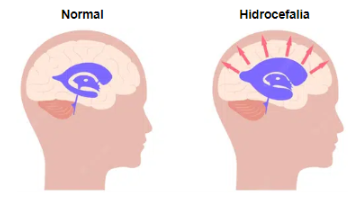
\includegraphics[width=0.8\textwidth]{img/comp_normal_hidro.PNG}
    \caption{Comparación entre cerebro normal e hidrocefálico \cite{comp_normal_hidrocefalia}}
    \label{fig:comp_normal_hidro}
\end{figure}

El LCR es un fluido corporal incoloro de composición similar a la del plasma producido por el plexo coroideo de los ventrículos laterales, red de vasos sanguíneos ubicadas en el interior de cada ventrículo (Figura \ref{fig:plexos_coroideos}), y reabsorbido por las vellosidades aracnoideas. El LCR actúa como un amortiguador con el fin de proteger al cerebro y a la médula espinal de posibles golpes. También participa en la eliminación de productos de desecho metabólicos, en el transporte de hormonas y nutrientes, proporciona soporte estructural y protección inmunológica y es esencial para el mantenimiento de la homeostasis\footnote{La homeostasis se define como la capacidad que tiene el cuerpo para regular y mantener constantes las condiciones internas, a pesar de las variaciones externas e internas \cite{homeostasis}.} en la médula y el cerebro.
\begin{figure}[h]
    \centering
    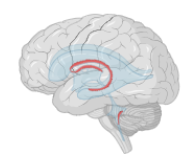
\includegraphics[width=0.6\textwidth]{img/plexos_coroideos.PNG}
    \caption{Plexos coroideos}
    \label{fig:plexos_coroideos}
\end{figure}

En circunstancias normales existe un equilibrio entre la producción y absorción de LCR, sin embargo cuando este balance está descompensado la cantidad de líquido cefalorraquídeo se acumulará en exceso produciendo un aumento de presión en el cerebro y causando diversos síntomas y complicaciones. Se considera que la PIC está en valores normales cuando oscila entre los 5-15 mmHg, si supera los 20 mmHg el paciente requiere de atención médica \cite{mmhg}.

Cabe destacar que los ventrículos cerebrales son cavidades dentro del cerebro que se conectan entre sí a través de canales estrechos por los que fluye el LCR. Hay cuatro ventrículos: dos de ellos se denominan “laterales”, son los más grandes y se encuentran ubicados en los hemisferios cerebrales. El tercer ventrículo está situado en el medio del cerebro, unido a los ventrículos laterales a través del orificio interventricular de Monro y conectado al cuarto ventrículo por medio del acueducto de Silvio. Este cuarto ventrículo se sitúa en la parte inferior del tronco cerebral, es decir, en la base del cerebro \cite{ventric}. 

Para una mejor comprensión visual, la Figura \ref{fig:anatomia_cerebro} nos muestra la disposición de las diferentes estructuras mencionadas en los párrafos anteriores.
\begin{figure}[h]
    \centering
    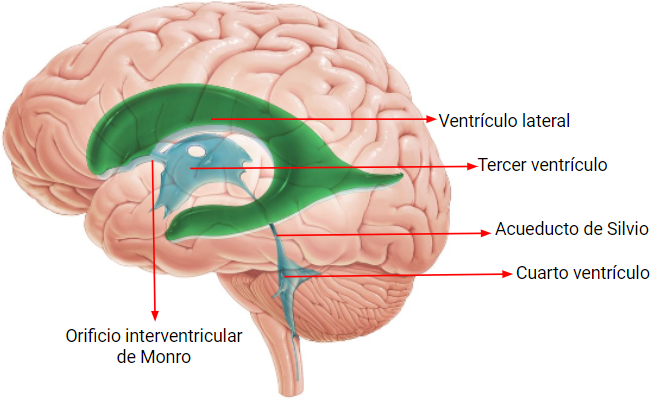
\includegraphics[width=0.9\textwidth]{img/anatomia_cerebro.PNG}
    \caption{Anatomía del cerebro}
     \cite{anatomia_cerebro}
    \label{fig:anatomia_cerebro}
\end{figure}

Dado el plano sagital de la Figura \ref{fig:anatomia_cerebro}, solo se puede ver un ventrículo lateral. Sin embargo, como mencionamos antes, hay dos, y el segundo se encuentra justo detrás del primero. En la Figura \ref{fig:ventrículos_laterales} podemos ver el conjunto del sistema ventricular cerebral desde otra perspectiva y observar claramente los dos ventrículos laterales.
\begin{figure}[h]
    \centering
    \includegraphics[width=0.6\textwidth]{img/ventrículos_laterales.PNG}
    \caption{Ventrículos laterales}
    \cite{ventriculos_laterales}
    \label{fig:ventrículos_laterales}
\end{figure}

\subsection{Causas y tipos}
La hidrocefalia puede ser congénita o adquirida. Esta podría ser una primera forma de clasificación basada en el momento de su aparición. Hablamos de hidrocefalia congénita cuando está presente desde el momento del nacimiento debido a malformaciones congénitas o complicaciones tanto del feto como del progenitor durante el periodo de gestación, mientras que el término hidrocefalia adquirida hace referencia, como su propio nombre indica, a la adquisición de esta en cualquier etapa de la vida y debido, por ejemplo, a traumatismos, derrames cerebrales, infecciones o tumores \cite{tipos_hidrocefalia}. 

En relación al flujo del líquido cefalorraquídeo, podemos distinguir dos tipos de hidrocefalia, comunicante y no comunicante u obstructiva.

En primer lugar tenemos la hidrocefalia comunicante. En este tipo de hidrocefalia se presentan alteraciones en la absorción de LCR en el espacio subaracnoideo, es decir, el flujo se ve bloqueado al salir de los ventrículos, en los que sí que puede fluir ya que se encuentran abiertos, de ahí recibe el nombre de comunicante. Esta alteración en el proceso de absorción tiene lugar en las vellosidades aracnoideas\footnote{Las vellosidades aracnoideas están formadas por células especializadas que absorben líquido cefalorraquídeo (LCR) del espacio subaracnoideo y lo devuelven al sistema venoso \cite{vellosidad}.}, encargadas de realizar correctamente esta función. Estas estructuras pueden verse afectadas por múltiples causas tales como traumatismos craneoencefálicos, hemorragias subaracnoideas, inflamaciones o cambios de presión que las van a impedir desempeñar su papel con normalidad viéndose disminuida su capacidad para reabsorber el LCR \cite{wiki_hidrocefalia}.

Por otra lado, la hidrocefalia no comunicante u obstructiva se da debido a una obstrucción que normalmente suele ser en el acueducto de Silvio. Las causas más comunes de la obstrucción suelen ser la estenosis del acueducto, malformación de Dandy-Walker y malformación de Chiari de tipo II. La estenosis del acueducto de Silvio es el estrechamiento congénito o adquirido de este canal. Cuando la estenosis es adquirida puede deberse a la presencia de un tumor, infección o hemorragia pero cuando es congénita suele ser por la presencia de síndromes o malformaciones genéticas. La estenosis de este acueducto cerebral es la causa más común de hidrocefalia congénita \cite{msd_hidrocefalia}.

En cuanto a las malformaciones de Dandy-Walker y Chiari tipo II, ambas son congénitas. La primera de ellas se desarrolla entre las semanas 7-10 del periodo de gestación y está caracterizada por la presencia de alteraciones en el correcto desarrollo del cerebelo, un aumento en el tamaño del cuarto ventrículo y la dilatación de la fosa posterior del cráneo, lo que puede provocar un aumento de la presión intracraneal, asociándose en el 70-90\% de los casos con hidrocefalia. Aunque su origen sigue siendo desconocido, se ha asociado en numerosas ocasiones con diferentes causas ambientales durante el embarazo y diversas alteraciones cromosómicas.  Esta malformación representa entre el 4-10\% de todos los casos de hidrocefalia, siendo su prevalencia de 1 de cada 25/30.000 casos con un frecuencia mayor en las mujeres en proporción de 3:1 respecto de los hombres \cite{aepnya_article}. 

La malformación de Chiari, o también conocida como malformación de Arnold Chiari, se trata de una afección congénita del cerebro en la cuál el cerebelo se encuentra desplazado hacia abajo adentrándose en el canal medular. Como consecuencia de este desplazamiento, se produce una presión anormal tanto en el cerebro como en la médula interfiriendo en el flujo normal de LCR. Esto lo podemos observar claramente en la Figura \ref{fig:chiari}, un caso de malformación de Chiari que presenta hidrocefalia. Aunque existen varios tipos de este defecto congénito, que probablemente no guardan relación los unos con los otros, los más comunes son el tipo I y tipo II \cite{stanford_chiari}. En este trabajo revisaremos la malformación de Chiari tipo II, ya que el 90\% de los casos están asociados con hidrocefalia y también con siringomielia, acúmulo de LCR en el interior de la médula espinal \cite{chiari_malformaciones}.


\begin{figure}[h]
    \centering
    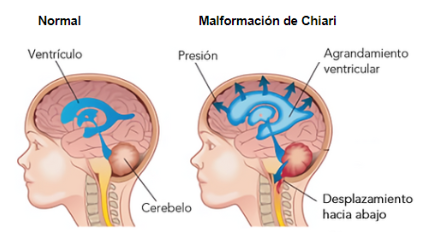
\includegraphics[width=0.9\textwidth]{img/Chiari.PNG}
    \caption{Comparación entre un individuo normal y otro con malformación de Chiari}
    \cite{chiari}
    \label{fig:chiari}
\end{figure}

En la malformación de Chiari tipo II, el desplazamiento del cerebelo es más pronunciado que en el tipo I causando así una mayor presión. Es común observar este tipo de malformación en bebés que presentan espina bífida, defecto congénito grave que afecta a la columna vertebral, debido a que esta no se forma y cierra como debería ocasionando graves daños en la médula espinal y nervios \cite{chiari_t2}. En la Figura \ref{fig:bebe_espina} podemos observar la apariencia de recién nacidos que presentan esta condición. 
\begin{figure}[h]
    \centering
    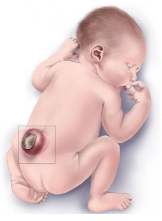
\includegraphics[width=0.35\textwidth]{img/bebe_espina.PNG}
    \caption{Recién nacido con espina bífida}
    \cite{espina_bifida}
    \label{fig:bebe_espina}
\end{figure}

Los tres tipos más comunes de espina bífida, de menor a mayor gravedad, son: espina bífida oculta, meningocele y mielomeningocele, siendo este último el más común en casos de malformación de Chiari tipo II \cite{mayo_chiari}. En la Figura \ref{fig:tipos_espina} vemos como la espina bífida oculta no presenta un “saco” o apertura en la espalda, la espina bífida se encuentra “escondida” y de ahí su nombre. En ocasiones el diagnóstico llega en edades más tardías, posteriores al nacimiento, ya que no suele provocar discapacidades debido a que tanto la médula espinal como los nervios suelen ser normales \cite{cdc_espina_bifida}. 

En el tipo meningocele y mielomeningocele sí que podemos observar esa protuberancia en la espalda. La diferencia entre estos dos tipos radica en que en la espina bífida meningocele, la médula espinal no se encuentra dentro de ese saco por lo que normalmente ni los nervios ni la médula suelen estar afectados y las discapacidades que puede ocasionar son menores respecto al tipo mielomeningocele. En esta última manifestación de espina bífida, parte de la médula espinal y los nervios se encuentran dentro de ese saco ocasionando numerosos daños y diversas discapacidades que pueden llegar a ser de gran gravedad \cite{cdc_espina_bifida}.
\begin{figure}[h]
    \centering
    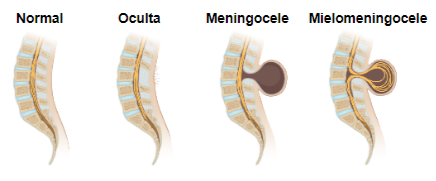
\includegraphics[width=0.9\textwidth]{img/tipos_espina.PNG}
    \caption{Tipos de espina bífida}
    \label{fig:tipos_espina}
\end{figure}

El último tipo de hidrocefalia es la denominada hidrocefalia normotensiva (HNT). Este tipo de hidrocefalia está caracterizada por el deterioro en el proceso de absorción de LCR y a diferencia de la hidrocefalia comunicante y obstructiva, el aumento de presión debido al incremento de LCR es muy pequeño o incluso nulo; se ve a menudo en adultos que superan los 60 años de edad y en numerosas ocasiones es diagnosticada de forma incorrecta, confundiendola con la enfermedad de Parkinson u otro trastorno neurológico relacionado con el envejecimiento \cite{elsevier_hidrocefalia_hnt}. 
En la mayoría de los casos de HNT, la causa del bloqueo en las vías de absorción del líquido cefalorraquídeo es desconocida, lo que lleva a clasificarla como idiopática. Cuando existe una causa identificable, como un trauma, tumor, accidente cerebrovascular o meningitis, se denomina HNT secundaria \cite{hnt-hidrocefalia-adultos}.

\subsection{Síntomas y complicaciones}
Para tratar los diversos síntomas que provoca la hidrocefalia, es interesante hacer una diferenciación entre bebés y niños pequeños con niños en edades más avanzadas y adultos.
En bebés y niños, los huesos del cráneo no están completamente fusionados, por lo que los signos de hidrocefalia pueden ser más notorios ya que la cabeza del bebé puede aumentar de tamaño, y la fontanela, área blanda de la cabeza del bebé, puede sentirse tensa o hinchada. La piel puede parecer estirada y brillante, y las venas en el cuero cabelludo pueden parecer más llenas o dilatadas de lo normal \cite{sint_niños}.

Entre los diversos síntomas que experimentan los bebés se incluyen:
\begin{itemize}
    \item Vómitos
    \item Alimentación deficiente
    \item Apatía
    \item Irritabilidad
    \item Desviación de los ojos hacia abajo
    \item Convulsiones ocasionales
\end{itemize}
En niños de edades más avanzadas podemos observar problemas de equilibrio, retraso en el desarrollo de procesos como caminar o hablar y un peor rendimiento escolar debido a la dificultad para concentrarse o recordar cosas.

Respecto a los adultos, los huesos del cráneo están completamente cerrados por lo que no vamos a notar ese aumento anormal del tamaño de la cabeza pero sí un incremento de la presión intracraneal debido al agrandamiento de los ventrículos \cite{sint_adult}.

Además de vómitos y apatía destacan otros síntomas como: 
\begin{itemize}
    \item Dolor de cabeza
    \item Cambios de personalidad
    \item Falta de coordinación
    \item Concentración deficiente
    \item Problemas visuales
    \item Fatiga
    \item Vértigos
\end{itemize}
Como en todas las patologías, la magnitud de los síntomas y su impacto difieren significativamente entre cada paciente. En el caso de síntomas persistentes durante un extenso periodo de tiempo, existe el riesgo de que el paciente desarrolle una discapacidad considerable. Se destaca la importancia de un diagnóstico temprano como un elemento crucial para abordar los síntomas de manera efectiva y lograr una resolución satisfactoria.

\subsection{Diagnóstico}
El diagnóstico prenatal de la hidrocefalia es fundamental para garantizar un manejo adecuado y planificar la atención médica necesaria tanto para el bebé como para la madre. Se realiza a través de una combinación de técnicas de imagen entre las que se incluyen la ecografía y la resonancia magnética (RMN) fetal. 

Durante el embarazo, la ecografía es la herramienta principal para la detección de diversas anomalías en el feto. Esta técnica de imagen emplea ondas sonoras de alta frecuencia (ultrasonidos), los cuales han demostrado ser inocuos y totalmente seguros durante el periodo de gestación. Se trata de un procedimiento seguro, no doloroso, rápido, con un coste inferior a otras pruebas diagnósticas y no invasivo en el que el ecografista le extenderá un gel sobre la piel, deslizando un instrumento llamado transductor para obtener así imágenes de estructuras internas de nuestro organismo \cite{eco}.

En el segundo trimestre de embarazo, se realiza una ecografía rutinaria que puede revelar la presencia del agrandamiento de los ventrículos del feto, signo temprano de hidrocefalia. Ante esta sospecha, está indicado realizar una resonancia magnética fetal, prueba diagnóstica que utiliza un campo magnético y ondas de radiofrecuencia para la obtención de imágenes más detalladas del feto. Al igual que la ecografía, no emplea radiaciones ionizantes (rayos X), es indolora y totalmente segura aunque su coste es más elevado y el tiempo de duración más prolongado, entre 20-60 minutos aproximadamente \cite{rmn_fetal}.

Este diagnóstico prenatal no siempre es definitivo. Tras el nacimiento, se requieren pruebas adicionales que confirmen el diagnóstico y evalúen la gravedad de la afección. Entre estas pruebas se encuentran diversos procedimientos de imagenología como la Tomografía Axial Computarizada (TAC, también conocido como TC o escáner), resonancia magnética (RMN) o ecografía transfontanelar. Tanto el TAC como la RMN son las pruebas diagnósticas que se emplean en los adultos, sin embargo la ecografía transfontanelar se realiza en recién nacidos o lactantes. Este tipo de prueba consiste en llevar a cabo una ecografía a través de las fontanelas, espacios entre los huesos del cráneo de un recién nacido, las cuales nos van a hacer de “ventana” para poder observar el cerebro y comprobar si existe dilatación ventricular \cite{eco_trans}. 

El TAC, se trata de una herramienta valiosa a la hora de diagnosticar numerosas patologías. Es una técnica de imagen avanzada que combina el uso de rayos X con tecnología de computadora (informática). En este examen médico, los rayos X se emiten desde distintos ángulos (a diferencia de una radiografía convencional en la que solo se emplea un único haz de rayos en una sola dirección) para formar así cortes-secciones del cuerpo del paciente (en este caso de la cabeza). Estos cortes se procesan en el ordenador teniendo como resultado imágenes detalladas de los órganos explorados. El empleo de radiación hace que la prueba no sea apta para determinados pacientes, por ejemplo para embarazadas ya que puede afectar de forma perjudicial al feto. En ocasiones, tanto para el TAC como para la RMN, se requiere del uso de un contraste intravenoso u oral para llevar a cabo el procedimiento con el objetivo de aumentar la visibilidad de ciertas estructuras \cite{tac}. 


\subsection{Tratamiento}

La hidrocefalia está caracterizada por tratarse de una afección crónica que actualmente no cuenta con una cura definitiva que revierta permanentemente el daño cerebral asociado. A pesar de la ausencia de una solución definitiva, es posible controlar y manejar de manera eficaz esta condición mediante una amplia variedad de tratamientos disponibles hoy en día. Todos estos tratamientos están diseñados para regular el flujo de líquido cefalorraquídeo en el cerebro con el fin de disminuir la presión intracraneal aliviando así los síntomas asociados. Principalmente destacan dos procedimientos: las derivaciones (shunts), tratamiento por excelencia y el que será revisado a lo largo de este apartado, y la ventriculostomía endoscópica del tercer ventrículo (VET). 

La ventriculostomía endoscópica del tercer ventrículo se trata de un procedimiento quirúrgico indicado para hidrocefalia obstructiva y concentrado en aliviar la presión ejercida por el LCR acumulado en exceso. Debido a que la mayoría de las obstrucciones se producen en el acueducto de Silvio o en el cuarto ventrículo, la ventriculostomía se realiza en el tercer ventrículo. Se realiza un pequeño agujero en el cráneo (trépano) y se introduce un endoscopio para hacer una perforación en la pared del tercer ventrículo y conseguir así una nueva vía de drenaje salvando la obstrucción \cite{vet}. 

Las válvulas de derivación son el principal tratamiento para la hidrocefalia. Estos dispositivos médicos permiten el drenaje del líquido cefalorraquídeo excedente hacia otra cavidad corporal donde pueda ser reabsorbido, consiguiendo así una disminución de la presión intracraneal. Una derivación consta de dos tubos delgados de diferente longitud, catéteres, conectados a una válvula unidireccional, encargada de regular la cantidad, la dirección de flujo y la presión de LCR fuera del sistema ventricular del cerebro \cite{derivacion}.

El catéter más corto, catéter proximal, se introduce en los ventrículos para recoger el exceso de líquido mientras que el catéter distal, el más largo, se coloca en la cavidad corporal donde ese excedente de LCR va a ser derivado para su absorción. En la Figura \ref{fig:valvula} podemos observar la apariencia de la válvula. 
\begin{figure}[h]
    \centering
    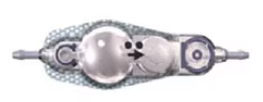
\includegraphics[width=0.7\textwidth]{img/valvula.PNG}
    \caption{Válvula}
    \cite{derivacion}
    \label{fig:valvula}
\end{figure}

La flecha negra nos indica la dirección del flujo, por lo tanto el catéter distal (o catéter largo) deberá ir colocado en el extremo al que apunta la flecha, según esta imagen en el extremo derecho, y el catéter proximal (o catéter corto) en el extremo opuesto. Algunas válvulas incluyen un reservorio que puede ser usado por el neurocirujano para diversos propósitos, por ejemplo, para probar la función de la derivación al purgarlo o para tomar una muestra de LCR \cite{derivacion}. En la Figura \ref{fig:colocacion_valvula} podemos ver donde estaría ubicada una vez que ha sido colocada.
\begin{figure}[h]
    \centering
    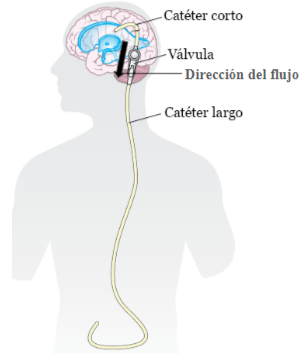
\includegraphics[width=0.7\textwidth]{img/Colocacion_valvula.PNG}
    \caption{Colocación de una válvula ventriculoperitoneal}
    \cite{colocacion_derivacion}
    \label{fig:colocacion_valvula}
\end{figure}

En función de la cavidad corporal donde va a ser derivado el excedente de LCR tenemos tres sistemas de derivación (Figura \ref{fig:derivaciones}):
\begin{itemize}
    \item Derivación ventriculoperitoneal (DVP), es la más común y el que revisaremos a lo largo de este trabajo, el LCR es desplazado desde los ventrículos hasta la cavidad peritoneal, ubicada en el abdomen 
    \item Derivación ventriculoatrial, empleado cuando no se puede usar una derivación ventriculoperitoneal debido a que el peritoneo ha perdido su capacidad absortiva \cite{elsevier_dva}, el LCR es desplazado desde los ventrículos hasta una cavidad del corazón, generalmente la aurícula derecha \cite{au_dcha} 
    \item Derivación lumboperitoneal, el LCR es desplazado desde la región lumbar hasta la cavidad peritoneal
\end{itemize}

\begin{figure}[h]
    \centering
    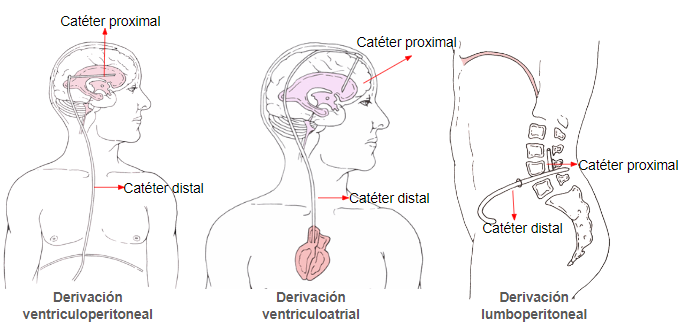
\includegraphics[width=1.2\textwidth]{img/derivaciones.PNG}
    \caption{Tipos de derivaciones}
    \cite{tipos_derivacion}
    \label{fig:derivaciones}
\end{figure}

El mecanismo de estos dispositivos es muy sencillo, cuando la presión intracraneal es baja, la válvula permanece cerrada y cuando ésta aumenta, la válvula se abre y permite que el LCR fluya hacia al peritoneo a través del catéter distal. A medida que el LCR es drenado, la presión disminuye cerrando de nuevo la válvula y cesando el flujo. Existen dos tipos de válvulas en función del mecanismo de regulación de LCR, válvulas de presión fija y de presión programable. Las de presión fija mantienen una tasa de flujo constante que viene dada por la configuración de un valor de presión determinado, es decir, a un valor de presión X la válvula se abre y el líquido se drena, mientras que las válvulas de presión programable o ajustable permiten modificar esta tasa de flujo en función de las necesidades del paciente en cada momento. Este ajuste se realiza de forma no invasiva mediante herramientas magnéticas durante tu cita médica, de forma que no requiere de otro procedimiento quirúrgico. Para llevarlo a cabo simplemente hay que localizar la válvula, colocar el instrumento sobre ella, leer la presión actual y realizar el ajuste, programando una nueva presión que se adapte a las necesidades del paciente.  En la Figura \ref{fig:ajuste_valvula} podemos observar como se realiza el ajuste, girando la herramienta hasta alcanzar el nivel de presión deseado.
\begin{figure}[h]
    \centering
    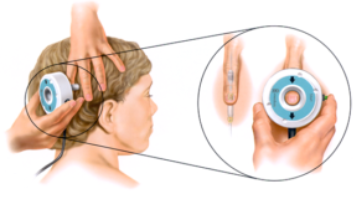
\includegraphics[width=0.7\textwidth]{img/ajuste_valvula.PNG}
    \caption{Ajuste de la válvula}
    \cite{herr_mag}
    \label{fig:ajuste_valvula}
\end{figure}

Según cada casa comercial, las válvulas tienen diferentes niveles de presión predefinidos, algunas presentan hasta 8. Cada nivel de presión se corresponde con una configuración que regula la cantidad de LCR  que se va a drenar en función de la presión intracraneal del paciente. Los niveles más bajos, por lo general, se utilizan en personas cuya PIC no es demasiado alta, es decir, presentan menos líquido acumulado por lo que la presión ejercida por éste es menor que en personas que retienen más LCR y necesitan que se drene más cantidad, por lo que se programa la válvula en niveles más altos. Esta correspondencia entre el nivel y la cantidad de líquido drenado en cada uno de ellos, viene recogida en una tabla como la de la Figura \ref{fig:tab_ajuste} que le servirá al neurocirujano para elegir el nivel de programación de la válvula en función de los niveles de presión intracraneal que presente el paciente.
\begin{figure}[h]
    \centering
    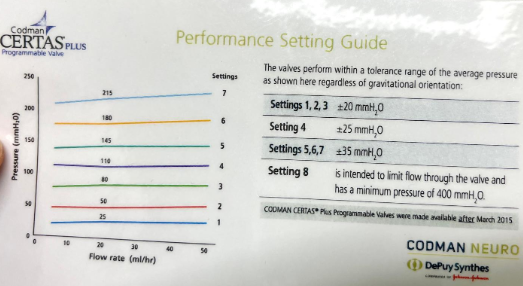
\includegraphics[width=0.9\textwidth]{img/tab_ajuste.PNG}
    \caption{Tabla de la válvula programable Codman CERTAS Plus. Imagen Propia }
    \label{fig:tab_ajuste}
\end{figure}

%\subsubsection{Sub Subsección}



\section{Estado del arte y trabajos relacionados}
En esta sección se procederá a realizar una revisión bibliográfica sobre estudios y proyectos relacionados con este trabajo que puedan ser de interés para el desarrollo del mismo, incluyendo un breve resumen de cada uno de ellos.

\subsection{Científicos proyectan un sensor de presión intracraneal conectado vía wifi \cite{curitibaa}}
Este proyecto está centrado en el desarrollo de un sensor invasivo capaz de suministrar información de la presión intracraneal (PIC) de un paciente en tiempo real y poder transmitirla mediante una conexión a internet vía wifi a los teléfonos y ordenadores de los profesionales sanitarios con el objetivo de conseguir un monitoreo permanente de la PIC. Los usuarios de este innovador dispositivo serían pacientes con afecciones neurológicas graves tales como hidrocefalia, traumatismos craneoencefálicos o accidente cerebrovascular (ACV) entre otros. En la Figura \ref{fig:sensor_curitiba} podemos observar el prototipo del sensor de Curitiba. La caja negra contiene el circuito electrónico, el sistema wifi y la batería; el tubo con el catéter recoge los datos de la PIC.
\begin{figure}[h]
    \centering
    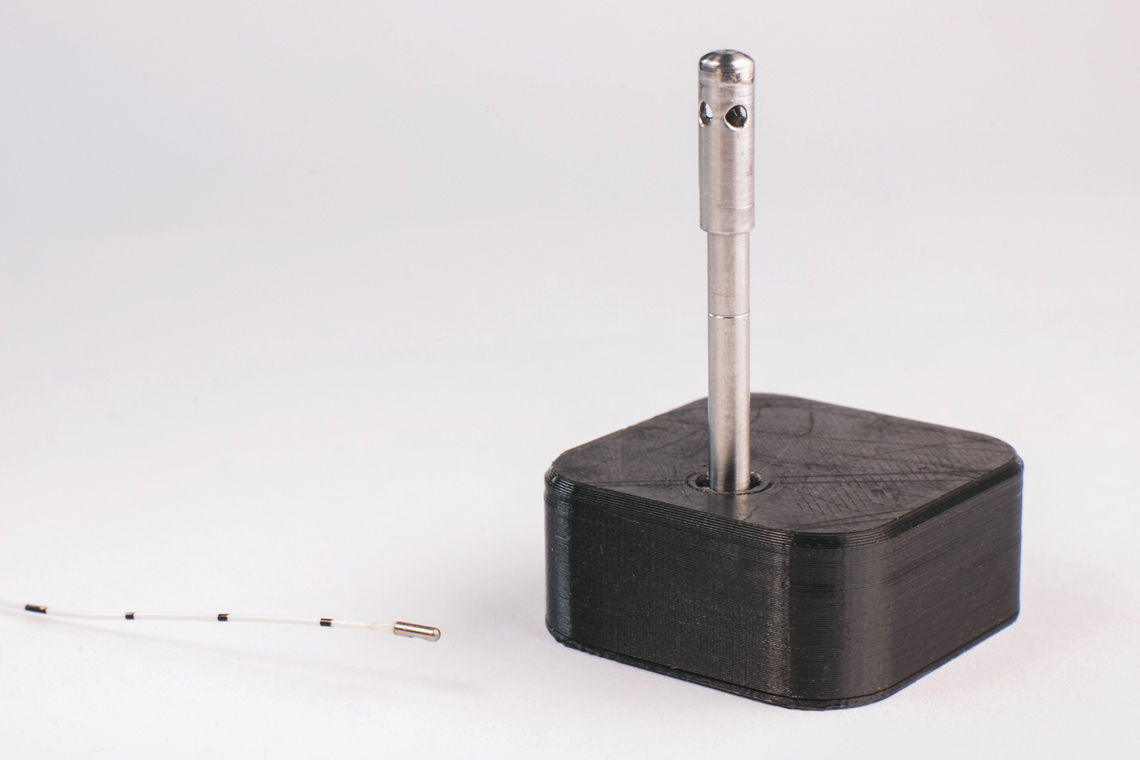
\includegraphics[width=0.7\textwidth]{img/curitiba.jpg}
    \caption{Prototipo del sensor de Curitiba}
    \cite{curitibaa}
    \label{fig:sensor_curitiba}
\end{figure}
Este sensor no se ve afectado ni por la posición ni por los movimientos del paciente ya que no se conecta por cable si no que los datos recopilados se transmiten por wifi a un servidor en la nube que será accesible por medio de una aplicación. Además, al estar desarrollado con fibra óptica no necesita ser retirado para llevar a cabo resonancias magnéticas ya que la fibra es inmune a las interferencias electromagnéticas.
En primer lugar, se realizó la validación en cerdos siendo el siguiente objetivo la evaluación en humanos. Si todo va correctamente se espera que en aproximadamente 5 años (el artículo fue publicado en 2023) el sensor se encuentre en el mercado y aunque su diseño está siendo sometido a una miniaturización y no se sabe con exactitud el coste de este dispositivo, se cree que puede rondar entre 1000 y 5000 reales (1000 reales son actualmente 179,07€), un precio que le permita competir con los sensores conectados por cable.
La investigación se realiza en la Universidad de Positivo, en la ciudad de Curitiba, capital del estado brasileño de Paraná y cuenta con la colaboración del Instituto de Neurología de Curitiba y de las empresas paranaenses Orakolo Tecnología y BMR Medical.

\subsection{Brain4care: monitorear la presión intracraneal sin perforación \cite{b4c_art}}
Brain4care se trata de una solución inalámbrica no invasiva que monitoriza las variaciones de la PIC a través de la forma de onda sustituta y la información de los parámetros asociados para interpretar cambios en pacientes con sospecha de alteración de la presión intracraneal \cite{b4c}. Como podemos observar en la Figura \ref{fig:b4c}, el dispositivo consiste en un sensor físico conectado a un dispositivo móvil vía Bluetooth que funciona a través de una aplicación IOS o Android. En este \href{https://youtu.be/9uHtUKreXvc}{enlace} podemos ver un vídeo que explica un poco el funcionamiento del dispositivo así como el informe que proporciona en base a los datos obtenidos.
\begin{figure}[h]
    \centering
    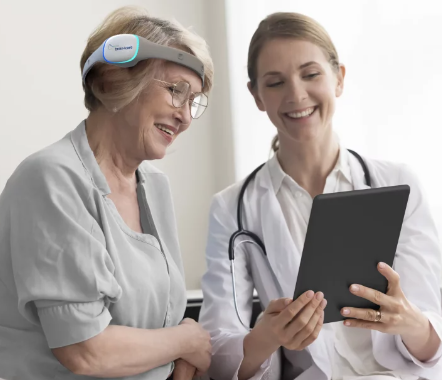
\includegraphics[width=0.7\textwidth]{img/b4c.PNG}
    \caption{Dispositivo Brain4care}
    \cite{b4c}
    \label{fig:b4c}
\end{figure}
La idea de este proyecto surge aproximadamente en 2005, cuando Sergio Mascarenhas de Oliveira, físico brasileño, es diagnosticado de hidrocefalia y tras su operación comienza a investigar diferentes formas para monitorear la forma de onda de la presión intracraneal de forma no invasiva. La forma de onda está correlacionada con la capacitancia cerebral (capacidad que presenta el cerebro para su expansión dentro del cráneo), condición fisiológica de suma importancia.
Este sistema hace uso de la Inteligencia Artificial para ayudar a interpretar las formas de las ondas y reconocer patrones de forma que los datos obtenidos permiten confirmar diagnósticos neurológicos incluso antes de que se manifiesten signos clínicos.

\subsection{SafeICP \cite{safeicp}}
El proyecto SafeICP es una iniciativa que busca el desarrollo de un monitor de presión intracraneal de bajo coste, fácil uso y de forma no invasiva permitiendo un seguimiento continuo y seguro del estado neurológico de los pacientes. Este dispositivo, potenciado por aprendizaje automático, ayudará a monitorizar patologías neuronales y ayudar en su diagnóstico y tratamiento valorando tanto los valores absolutos como las alteraciones de la presión intracraneal (PIC) \cite{safe}. Contará con un diseño que parte de los últimos avances científicos en el ámbito de la biofotónica para monitorizar a través de láser los niveles de PIC y del aprendizaje automático, subcampo de la inteligencia artificial. 
SafeICP es liderado por el Instituto de Ciencias Fotónicas (ICFO), con la participación  del Departamento de Tecnologías de la Información y las Comunicaciones (DTIC) de la Universidad Pompeu Fabra (UPF) y el Vall d’Hebron Instituto de Investigación (VHIR). También cuenta con la colaboración de la empresa ProCareLight, especializada en técnicas láser, y del Hospital Universitario Vall d’Hebron.

\subsection{Neurovent-P-tel \cite{raumedic}}
Raumedic ha desarrollado un sistema de medición inalámbrico de la presión intracraneal denominada Neurovent-P-tel (Figura \ref{fig:neurovent}), que surge como alternativa a los catéteres tradicionales con cable de monitorización de PIC. 
\begin{figure}[h]
    \centering
    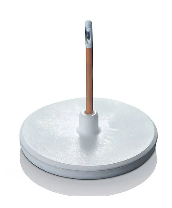
\includegraphics[width=0.3\textwidth]{img/neurovent.PNG}
    \caption{Neurovent-P-tel}
    \cite{raumedic}
    \label{fig:neurovent}
\end{figure}
Este sistema emplea tecnología de telemetría se implanta debajo del cuero cabelludo en el hueso craneal y permite recopilar mediciones de la presión intracraneal en el parénquima \footnote{Tejido funcional de un órgano, en este caso del cerebro. Esta compuesto por neuronas y células gliales \cite{parenquima}} cerebral de manera inalámbrica. Neurovent-P-tel mide la PIC mediante tecnología de microchip transfiriendo los valores de presión a un lector (Figura \ref{fig:readertdt1}) empleando principios RFID \footnote{Identificación por Radio Frecuencia (RFID), tecnología que permite identificar objetos mediante ondas de radio de manera única y pudiendo captar cientos de objetos a la vez \cite{rfid}} validados. 
\begin{figure}[h]
    \centering
    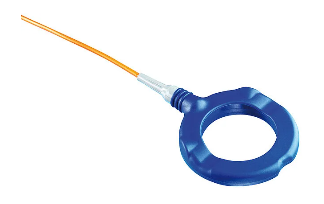
\includegraphics[width=0.5\textwidth]{img/readertdt1.PNG}
    \caption{Reader TDT1 readP}
    \cite{raumedic}
    \label{fig:readertdt1}
\end{figure}
Los datos recogidos se pueden almacenar en dispositivos como el RAUMED NeuroSmart y el MPR1 DATALOGGER o el RAUMED Home ICP. Este último es utilizado en el domicilio del paciente de forma continua y durante actividades cotidianas mientras que RAUMED NeuroSmart y MPR1 DATALOGGER se emplean en pacientes hospitalizados durante el tiempo que dure el ingreso.

Algunas de las ventajas que presenta esta solución son:
\begin{itemize}
    \item Comunicación inalámbrica con el catéter
    \item Datos registrados en RAUMED Neuro Smart, MPR1 DATALOGGER o RAUMED Home ICP
    \item Monitoreo móvil de pacientes en un campo hospitalario o ambulatorio
    \item Riesgo mínimo de infección
    \item Reducción de la estancia hospitalaria
\end{itemize}



\capitulo{4}{Metodología}

\section{Descripción de los datos}
Para el desarrollo de este proyecto no se han empleado datos ya existentes. Al ejecutar el programa, este nos solicita cuatro datos: nombre completo, año de nacimiento, usuario y contraseña. Una vez estos datos estén completos, el sensor comenzará a realizar lecturas de los valores de presión. Para más información consultar \textit{Anexo D}. En el futuro, cuando se pueda desarrollar la idea de este proyecto se generarán multitud de datos, desde los datos personales del paciente (nombre, apellidos, fecha de nacimiento, número de historia clínica etc) que deberán estar correctamente protegidos con las leyes vigentes del momento (contemplar \textit{Anexo A}), como todos los datos relativos a la presión intracraneal del paciente, que estará continuamente monitorizado. Todos estos datos estarán almacenados en historiales para poder analizarlos, realizar estadísticas y establecer patrones con el objetivo de mejorar la evolución del paciente.
 
\section{Técnicas y herramientas}

El objetivo de esta sección es hacer una breve recopilación tanto de las técnicas y aplicaciones empleadas para desarrollar este proyecto como de las herramientas necesarias para ello.

\subsection{Aplicaciones}

A continuación se presentan las aplicaciones gratuitas empleadas para desarrollar este trabajo acompañadas de una breve descripción de cada una de ellas. Algunas como Overleaf, GitHub o Arduino, han sido utilizadas a lo largo del grado.

\begin{itemize}
    \item \textbf{Overleaf} \cite{overleaf}: es una plataforma colaborativa en línea que utiliza LaTex para la publicación y redacción de documentos. LaTex es una herramienta para componer textos de aspecto profesional convirtiendo un documento de texto sin formato formado por comandos LaTex y texto en un archivo PDF. Para llevar a cabo esta conversión, LaTex emplea un software denominado motor TeX por lo tanto el usuario solo debe centrarse en el contenido del documento sin preocuparse de la apariencia visual. En este proyecto se ha empleado para desarrollar este documento y los anexos.
    
    \item \textbf{GitHub} \cite{github}: es una plataforma en línea gratuita de desarrollo de software colaborativo que utiliza el sistema de control de versiones Git cuya función es realizar un seguimiento de los cambios que se producen en los archivos. Es de código abierto y permite a los usuarios trabajar juntos en proyectos de software, facilitando el seguimiento de posibles cambios en el código, colaboración en equipo y organización de proyectos. Para este proyecto se ha creado un repositorio público en el que a través de tareas (issues) se ha ido organizando el desarrollo del mismo.
    
    \item \textbf{Arduino} \cite{arduino}: es una plataforma de código abierto basada en hardware y software libre. Es flexible, fácil de usar y de bajo coste, por lo que habitualmente es elegida para llevar a cabo distintos proyectos electrónicos. Arduino cuenta con un entorno de programación, Arduino IDE, con el que el usuario puede crear diferentes aplicaciones para las placas dándole todo tipo de utilidades. Esta placa puede ser programada tanto en Windows como en macOS y GNU/Linux y emplea un lenguaje de programación similar a C++ pero simplificado. Arduino ha sido elegido para realizar este proyecto principalmente por su sencillez y bajo coste.
    
    \item \textbf{Biorender} \cite{biorender}: es un programa online gratuito para elaborar imágenes científicas. En este proyecto se ha utilizado para crear alguna imagen como por ejemplo la Figura \ref{fig:tipos_espina}.

    \item \textbf{Unfold} \cite{unfold}: es un aplicación de edición de fotos y vídeos que se ha empleado para elaborar los vídeos contenidos en la carpeta demostraciones del \href{https://github.com/CeliaValladolid/TFG_Valvula_Derivacion_VentriculoPeritoneal}{Repositorio}.
    
\end{itemize}

\subsection{Herramientas}
Al igual que en el apartado anterior, se citarán las herramientas necesarias para llevar a cabo este proyecto así como un breve resumen de todas ellas.

\begin{itemize}
    \item \textbf{Placa de arduino UNO R3} \cite{placa}: es una placa de desarrollo de código abierto que integra un microcontrolador ATmega328P de alta eficiencia \cite{placa}. En la Figura \ref{fig:placa_Arduino} podemos observar la placa empleada para el proyecto junto con la indicación de cada uno de sus componentes.
    \begin{figure}[h]
    \centering
    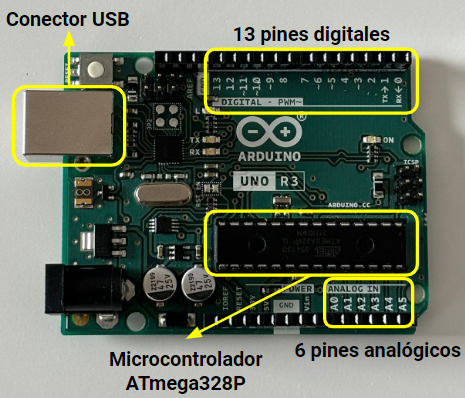
\includegraphics[width=0.6\textwidth]{img/PLACAPARTES.PNG}
    \caption{Placa de Arduino UNO R3. Imagen Propia}
    \label{fig:placa_Arduino}
\end{figure}

    \item \textbf{Cables}: cables empleados para realizar el cableado del proyecto, de la placa de Arduino a la protoboard o a los componentes que sea necesario. Hemos empleado cables macho-hembra\footnote{Los cables macho-hembra son cables que presentan un pincho en un lado y un hueco en el otro \cite{cables}} para llevar a cabo algunas conexiones. Podemos observarlos en la Figura \ref{fig:cables}.
    \begin{figure}[h]
    \centering
    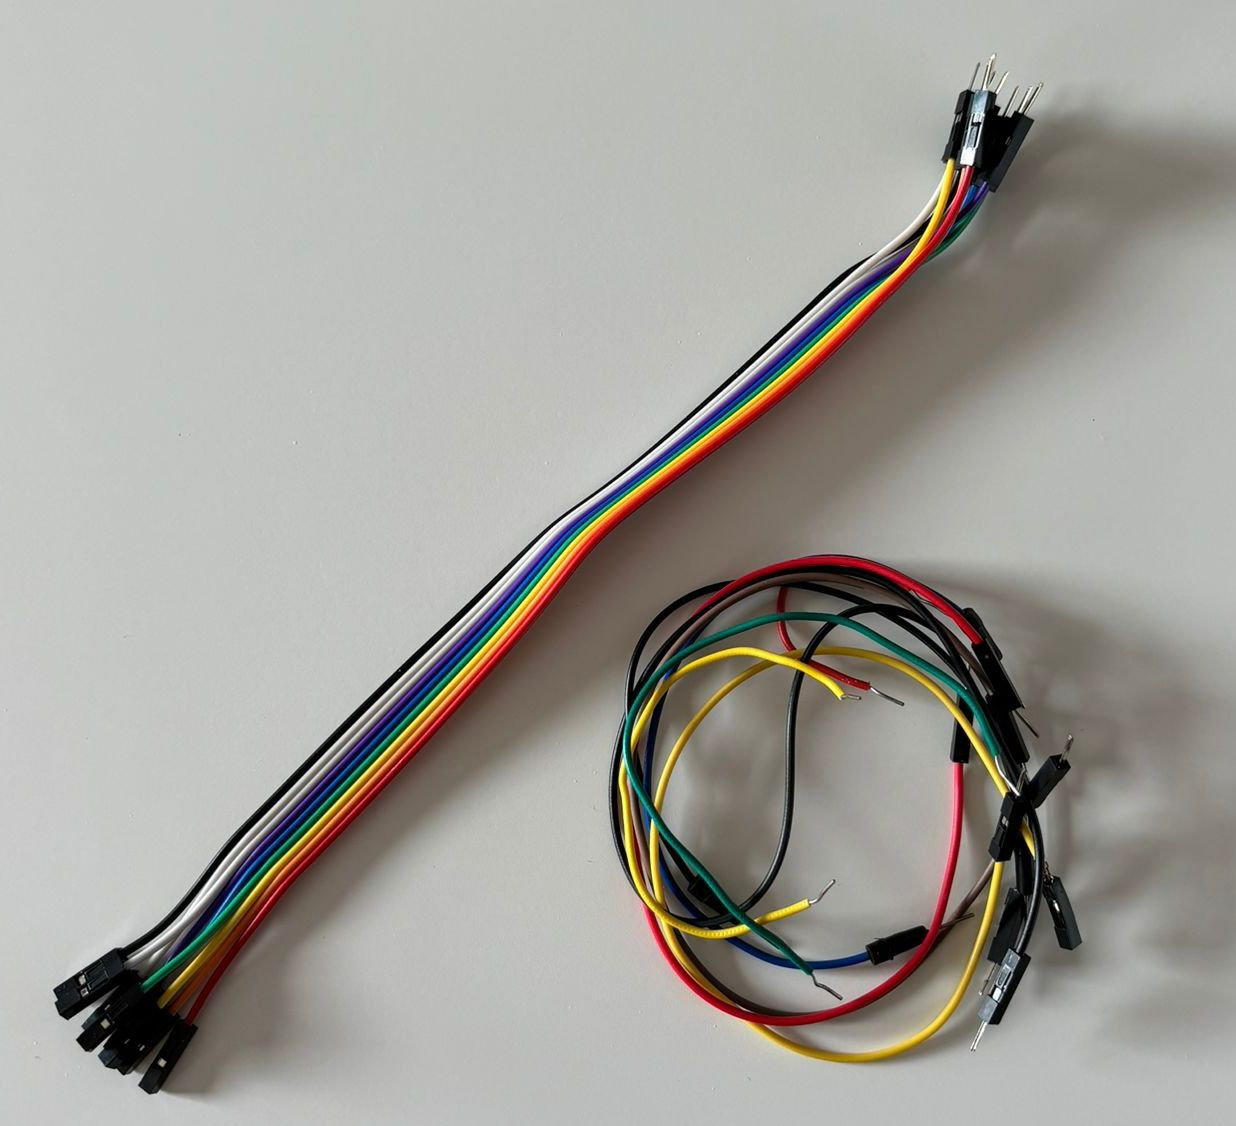
\includegraphics[width=0.6\textwidth]{img/cables.jpg}
    \caption{Cables. Imagen Propia}
    \label{fig:cables}
\end{figure}

    \item \textbf{ProtoBoard}: también conocida como placa de pruebas, se trata de una placa electrónica cuya función es el prototipado de circuitos y conexiones. Una protoboard consta de un número variable de clavijas (según el tamaño escogido) en las cuáles se insertan los diferentes componentes electrónicos y de 4 filas , dos superiores y dos inferiores, marcadas con el signo + y - encargadas de llevar la corriente y la toma tierra al circuito. Todos los pines de las diferentes filas están conectados entre sí. En la Figura \ref{fig:protoboard} podemos observar el aspecto de este componente.
    \begin{figure}[h]
    \centering
    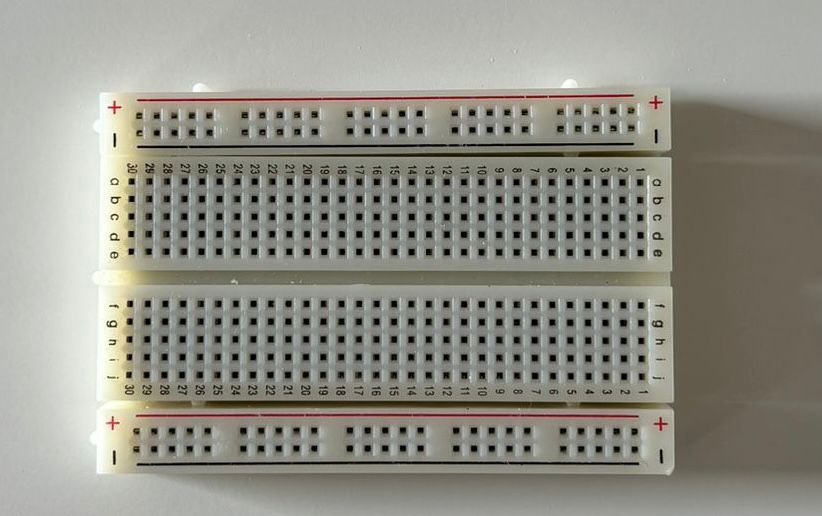
\includegraphics[width=0.6\textwidth]{img/proto.jpg}
    \caption{ProtoBoard, placa de pruebas. Imagen Propia}
    \label{fig:protoboard}
\end{figure}

    \item \textbf{Cable USB}: cable que permite conectar la placa de Arduino con un ordenador y así ejecutar las instrucciones programadas. Lo podemos observar en la Figura \ref{fig:USB}.
    \begin{figure}[h]
    \centering
    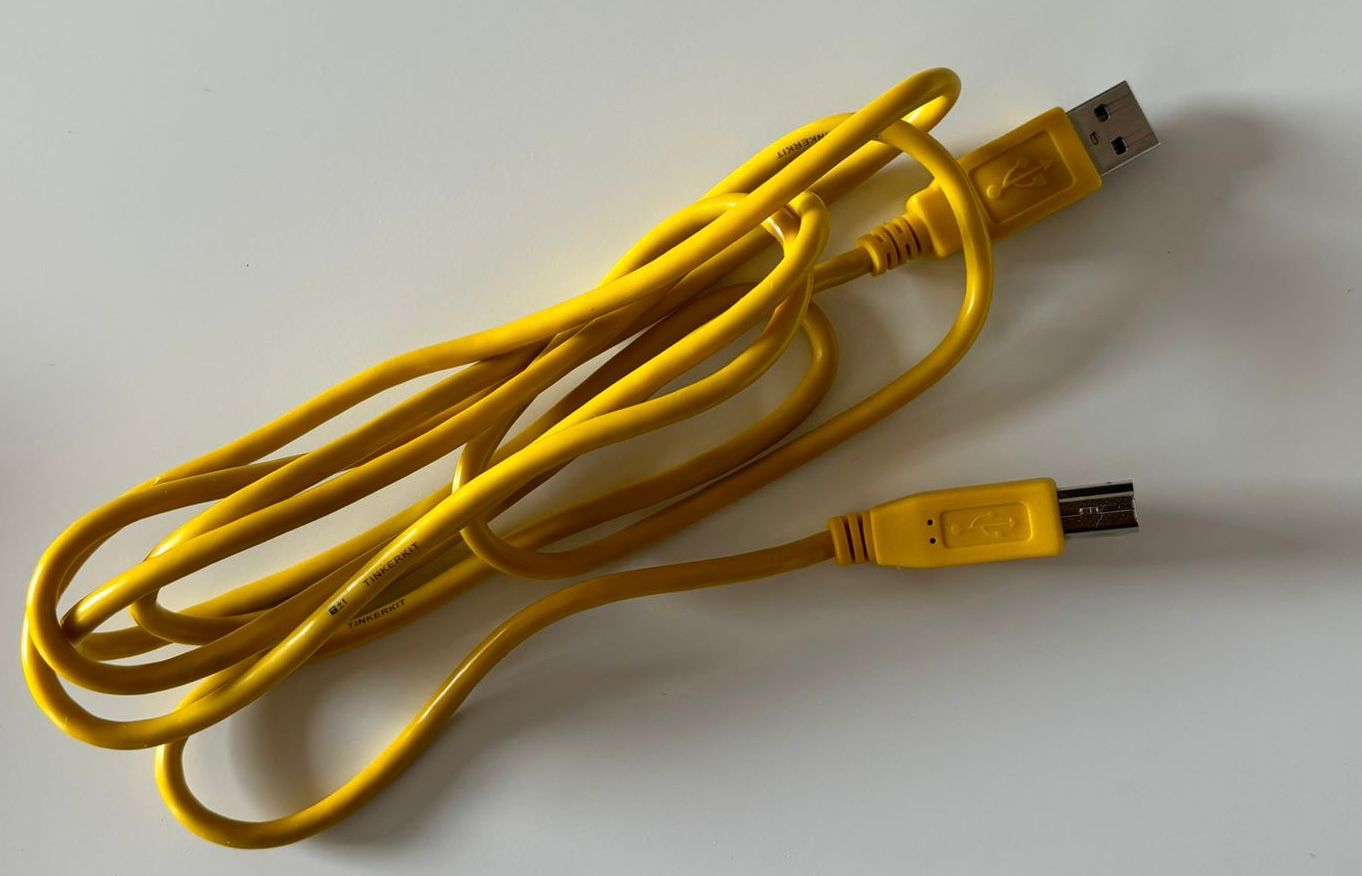
\includegraphics[width=0.6\textwidth]{img/usb.jpg}
    \caption{Cable USB. Imagen Propia}
    \label{fig:USB}
\end{figure}

    \item \textbf{Sensor de presión NPX MPX5010DP}: se trata de un sensor de presión diferencial de silicio integrado de doble puerto en un encapsulado SIP de 6 pines \cite{npx}. Según la Figura \ref{fig:sensor_pres} el pin 1 es el de la izquierda, el que presenta una muesca y el que se conecta a un pin analógico de nuestro Arduino. Los pines 2 y 3 son los que están a continuación y se conectan a GND y 5V respectivamente. Este sensor entrega en su salida un voltaje de 0-5 V, lo que le hace ideal para microcontroladores \cite{npx_}. 
    \begin{figure}[h]
    \centering
    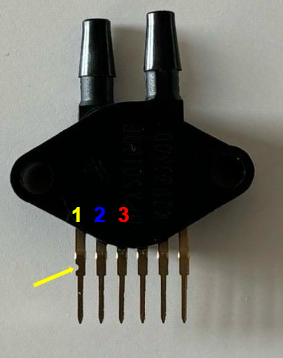
\includegraphics[width=0.35\textwidth]{img/sensor_1.PNG}
    \caption{Sensor de presión NPX MPX5010DP. Imagen Propia}
    \label{fig:sensor_pres}
    \end{figure}
    En la Tabla \ref{tab:caracteristicas_sensor} podemos ver recogidas las principales características del sensor:
    
    \begin{table}[htbp]
    \centering
    \begin{tabular}{>{\raggedright\arraybackslash}p{0.9\linewidth}}
    \hline
    \rowcolor{blue!20}
    \multicolumn{1}{c}{\textbf{Características del sensor NPX MPX5010DP}} \\
    \hline
    Calibración, compensación de temperatura y acondicionamiento de señal en chip \\
    Configuración diferencial \\
    Error máximo de 5,0\% entre 0°C y 85°C \\
    Diseño de una pieza de epoxi duradera \\
    Compensación de temperatura de -40°C a 125°C \\
    Galga extensiométrica de esfuerzo cortante de silicio patentada \\
    Rango de presión de 0KPa a 10KPa \\
    Rango de tensión de alimentación de 4,75VDC a 5,25VDC \\
    Sensibilidad de 450mV/mm \\
    Tiempo de respuesta de 1ms \\
    \hline
    \end{tabular}
    \caption{Características del sensor NPX MPX5010DP \cite{npx}}
    \label{tab:caracteristicas_sensor}
    \end{table}
    

    \item \textbf{Mini bomba}: mini bomba de agua sumergible que presenta un voltaje DC 3-5V y una corriente de 100-200 mA. Viene acompañada de una manguera de plástico para que circule el agua de un recipiente a otro. Ambos elementos los podemos observar en la Figura \ref{fig:mini_bomba}.
    \begin{figure}[h]
    \centering
    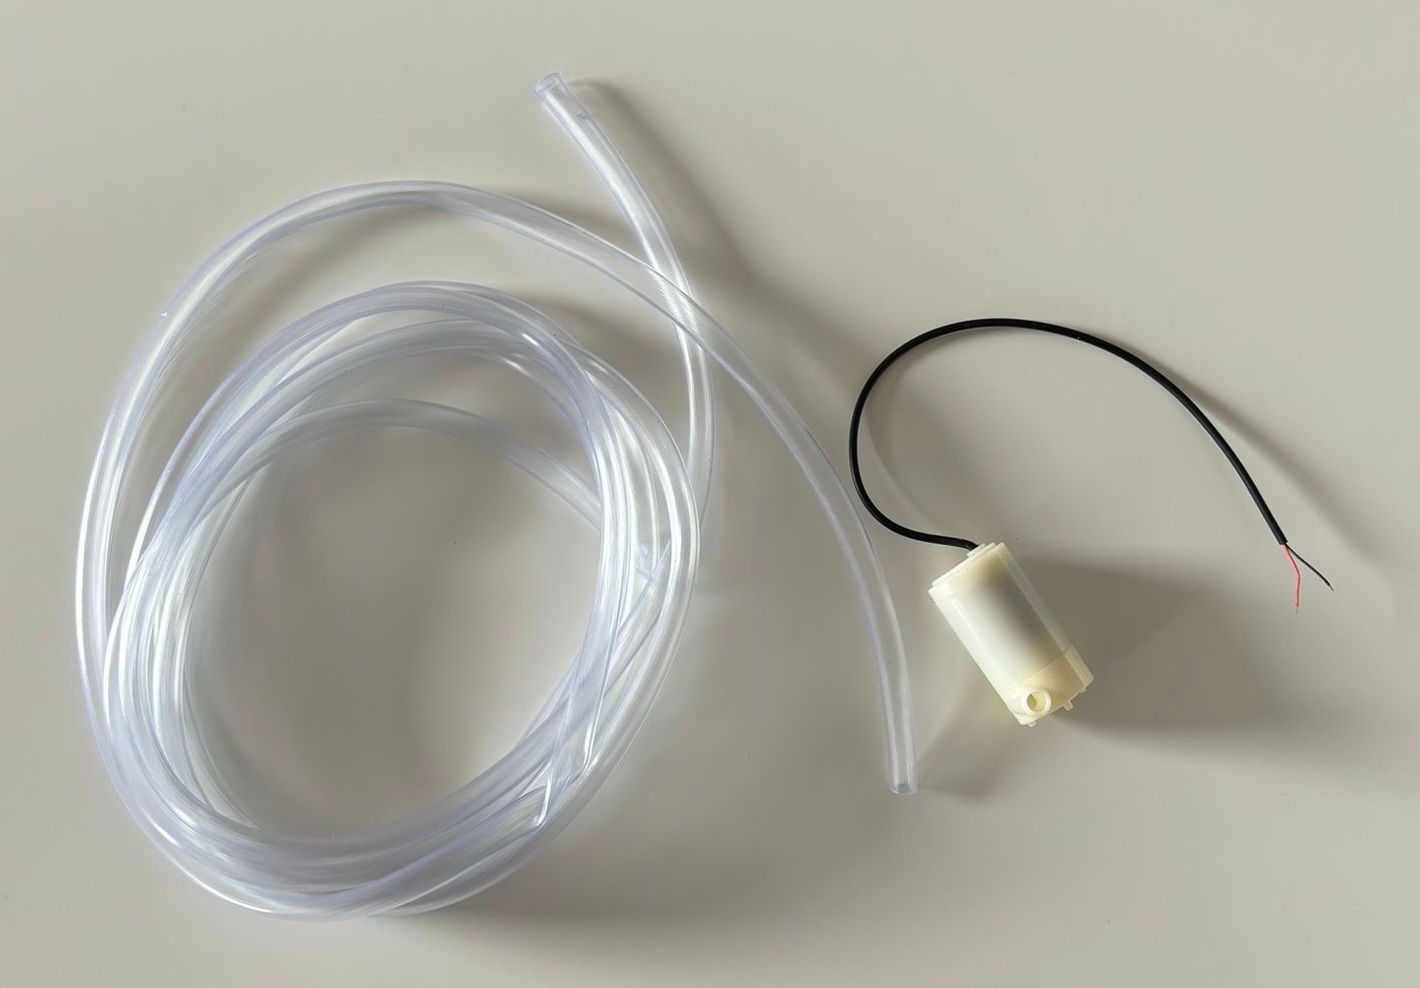
\includegraphics[width=0.65\textwidth]{img/bomba.jpg}
    \caption{Mini bomba. Imagen Propia}
    \label{fig:mini_bomba}
\end{figure}

    \item \textbf{Relé}: es un componente electromagnético que actúa como un interruptor, permitiendo el paso de la corriente cuando se encuentra cerrado e interrumpiendo este flujo cuando permanece abierto. Este dispositivo no se acciona de forma manual sino a través de una señal eléctrica. En su interior cuenta con una bobina conectada a la corriente y cuando ésta se acciona genera un campo electromagnético que provoca el cierre del contacto del relé, permitiendo así que circule la corriente. Cuando dejamos de suministrar corriente a la bobina, el contacto se abre,desaparece el campo electromagnético y el dispositivo que estamos controlando queda privado de corriente para seguir en funcionamiento \cite{rele}. En este proyecto emplearemos un relé de un canal para activar y desactivar la mini bomba. En la Figura \ref{fig:rele} podemos observar los pines y contactos con los que cuenta.
    \begin{figure}[h]
    \centering
    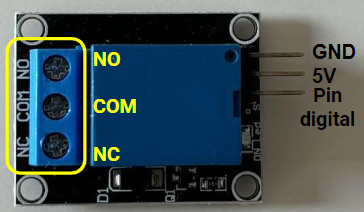
\includegraphics[width=0.6\textwidth]{img/relepartes.PNG}
    \caption{Relé. Imagen Propia}
    \label{fig:rele}
\end{figure}

    \item \textbf{Portapilas}: compartimento para albergar tres pilas en serie de 1,5V cada una consiguiendo así un voltaje total de 4,5V para poder alimentar nuestro circuito. Es apto para pilas LR6 AA (FR6, HR6, LR6) e incluye un interruptor ON/OFF. Lo podemos observar en la Figura \ref{fig:portapilas}.
    \begin{figure}[h]
    \centering
    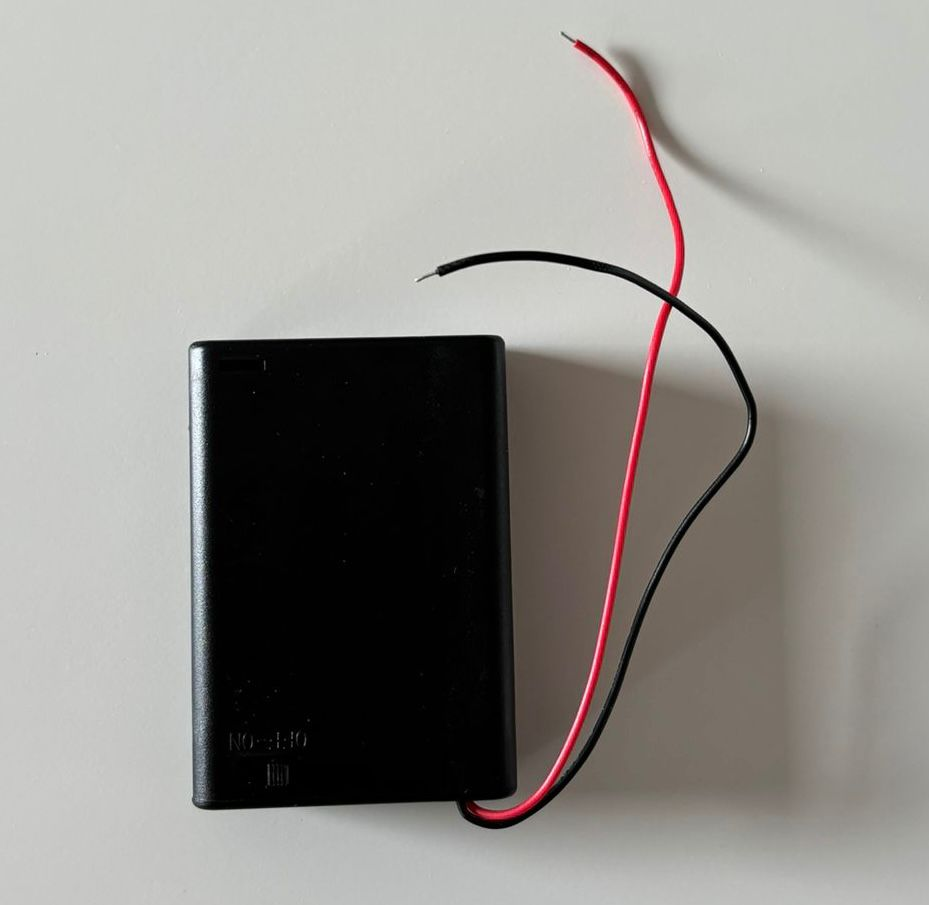
\includegraphics[width=0.6\textwidth]{img/portapilas.jpg}
    \caption{Portapilas. Imagen Propia}
    \label{fig:portapilas}
\end{figure}

    \item \textbf{Pilas}: pilas LR6 AA empleadas para alimentar nuestro circuito. Las podemos observar en la Figura \ref{fig: pilas}.
    \begin{figure}[h]
    \centering
    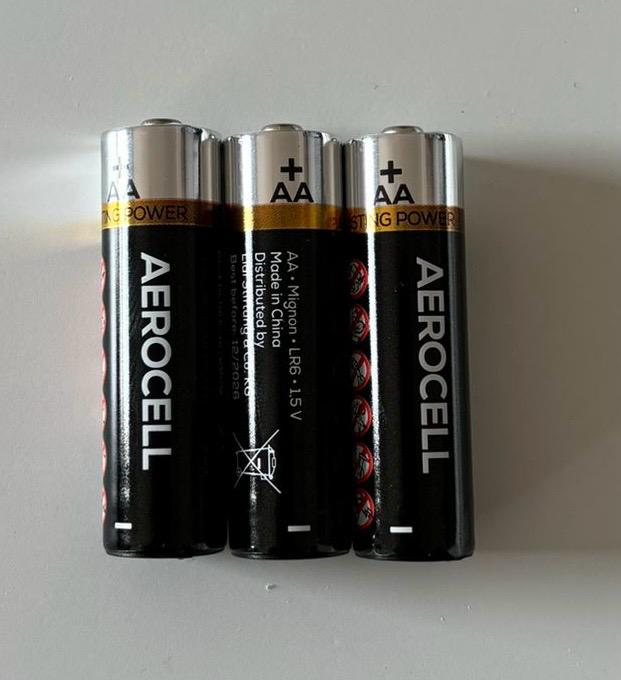
\includegraphics[width=0.5\textwidth]{img/pilas.jpg}
    \caption{Pilas. Imagen Propia}
    \label{fig: pilas}
\end{figure}

\end{itemize}

\capitulo{5}{Conclusiones}


\section{Resumen de resultados}
Los resultados obtenidos han sido satisfactorios, se ha cumplido el objetivo principal de este Trabajo de Fin de Grado, se ha logrado simular la funcionalidad de una válvula ventriculoperitoneal. Esta válvula es un dispositivo médico utilizado para derivar el exceso de líquido cefalorraquídeo (LCR) desde el sistema ventricular del cerebro hasta el peritoneo (para más información consultar la sección de \textit{Conceptos teóricos}), lo que ayuda a aliviar la presión intracraneal elevada. En este proyecto, se ha replicado este proceso mediante un sistema compuesto por un relé, un sensor de presión, y una mini bomba, verificando que todos los componentes funcionaban de forma correcta antes de montar el circuito completo. En el \textit{Anexo G} podemos encontrar las pruebas realizadas con el relé y el sensor, junto con el código necesario para su ejecución.


El montaje consiste en un recipiente que representa el cráneo, en cuyo interior podemos encontrar el sensor y la mini bomba. Al añadir agua a este recipiente, la presión aumenta, y este cambio será detectado por el sensor. Cuando la presión alcanza un umbral predeterminado, el relé activará la mini bomba, permitiendo el paso del líquido a otro recipiente, que simulará el peritoneo. En la Figura \ref{fig:proyect-realiad} podemos observar el montaje.

\begin{figure}[h]
    \centering
    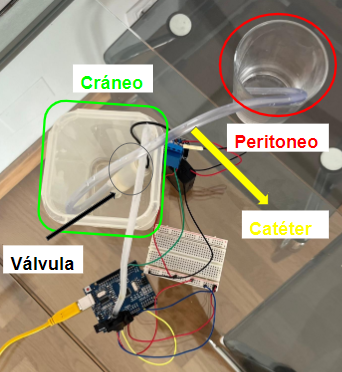
\includegraphics[width=0.7\textwidth]{img/proyect-realidad.PNG}
    \caption{Identificación de los componentes con el cuerpo humano. Imagen propia.}
    \label{fig:proyect-realiad}
\end{figure}

\newpage

\section{Discusión}
Como he mencionado anteriormente, los resultados han sido los esperados. No obstante, cabe destacar algunos detalles. En el código, el valor de presión predeterminado para que se active el relé es de 4 mmHg, y en el cuerpo humano entre 5-15 mmHg se consideran valores normales, no se requiere de atención médica hasta que no se alcancen los 20 mmHg. En este trabajo, se ha elegido el valor de 4 mmHg debido al recipiente empleado, se necesitaría un recipiente más alto y grande para lograr presiones de 20 mmHg. El problema radica en la limitación presentada por los cables. El cable de la mini bomba es demasiado corto para introducirlo en un recipiente más alto ya que se introduciría también el relé al que está conectado. Aún así el programa sería el mismo, salvo el valor de presión preestablecido. 

\section{Aspectos relevantes}

A lo largo de la elaboración de este proyecto se pueden destacar varios aspectos relevantes. 

En primer lugar, la identificación de carencias en el campo de la neurocirugía, la falta de dispositivos que empleen la telemetría\footnote{La telemetría es una tecnología de medición remota que permite recoger, procesar y transmitir la información de un dispositivo electrónico a otro\cite{telemetria}} para dar solución a diferentes problemas dentro de este área. A través de plataformas como Arduino y la selección de diferentes componentes electrónicos, se ha simulado la funcionalidad de una válvula de derivación, implementando un sistema automatizado que ajuste su apertura en base a las lecturas del sensor. Este sistema de regulación brinda una solución más precisa y personalizada, ya que la válvula está controlada en todo momento, ajustándose a las necesidades que requiera cada paciente. 

Además, se plantea el desarrollo de una aplicación móvil para conseguir monitorizar a los pacientes y controlar el dispositivo de una forma no invasiva, lo cual se convierte en un aspecto clave para lograr un manejo eficiente del dispositivo. Uno de los objetivos principales de este proyecto radica en la importancia de la medicina personalizada\footnote{La medicina personalizada busca el tratamiento adecuado a cada paciente sobre la base del diagnóstico preciso, las terapias dirigidas y el análisis de los datos \cite{med_per}.} ya que cada persona es diferente y por lo tanto las soluciones deben de estar enfocadas en ceñirse lo máximo posible al perfil de cada paciente. La aplicación permitirá realizar ajustes específicos del dispositivo basándose en las necesidades individuales y consiguiendo así mejorar de forma exponencial los resultados clínicos y la calidad de vida del paciente.

Este proyecto ofrece una base sólida para futuras investigaciones en el campo de la neurocirugía y la tecnología, abriendo nuevas puertas a diferentes soluciones y mejoras en el tratamiento de la hidrocefalia. Combina conocimientos de diferentes campos tales como la neurocirugía, ingeniería de la salud y desarrollo de software entre otros, mostrando la importancia del trabajo conjunto de diferentes áreas para conseguir dar solución a diferentes problemas en el ámbito de la medicina.

En resumen, estos serían los aspectos más relevantes del proyecto:
\begin{enumerate}
    \item Identificación de carencias en la Neurocirugía
    \item Aplicación práctica de la tecnología
    \item Sistema Automatizado
    \item Medicina Personalizada
    \item Base para futuros proyectos
    \item Interdisciplinariedad
\end{enumerate}








\capitulo{6}{Líneas de trabajo futuras}

Este apartado está dedicado a exponer algunas características y funcionalidades que han ido surgiendo a lo largo de la realización de este proyecto. El objetivo de todas ellas es mejorar aspectos como la seguridad, eficacia y versatilidad de este futuro dispositivo, consiguiendo así una solución más avanzada y completa.

Como he comentado en apartados anteriores, se trata de un dispositivo invasivo, colocado en el interior del cráneo a través de un procedimiento quirúrgico para monitorizar directamente la presión de LCR en mmHg\footnote{El milímetro de mercurio (mmHg) es una unidad de presión manométrica, es decir, medida en relación a la presión del ambiente con respecto a la atmósfera \cite{presion}.} Uno de los objetivos principales en cuanto al diseño es la miniaturización del dispositivo, conseguir que sea lo más pequeño posible para la máxima comodidad del paciente.

%https://www.essalud.gob.pe/ietsi/PETITORIO_DE_MATERIAL_MEDICO/pdf/MM-538.pdf 
Respecto a los materiales empleados, deben de ser compatibles con la realización de una RMN, es decir, no se pueden emplear metales ya que los imanes de la resonancia se sentirán atraídos por estos, interfiriendo posteriormente en los resultados. Solo algunos como el cobre, cobalto, cromo y titanio son metales seguros que no distorsionan el resultado. El titanio es un metal que se utiliza de forma habitual en dispositivos médicos implantables debido a que presenta una elevada resistencia a la corrosión de los fluidos corporales. Es biocompatible con los tejidos del organismo, no los daña ni produce toxicidad \cite{titanio}. Para los catéteres, el material más empleado es la silicona. Este material al igual que los demás ha sido previamente testado y es de gran calidad, hipoalergénico\footnote{Un material hipoalergénico o hipoalérgico es aquel que produce una reacción alérgica escasa o nula \cite{hipoalergenico}.}, antibacteriano, flexible, resistente y libre de látex y de toxinas \cite{silicona}. Una caracterítica destacable tanto de los catéteres como de la válvula es que sean radiopacos, es decir, que ofrezcan resistencia al ser atravesados por rayos X, u otra forma de radiación ionizante, de tal forma que en el resultado se vean de color blanco. Esta cualidad resulta interesante ya que permite a los neurocirujanos visualizar estos dispositivos de forma clara durante intervenciones guiadas radiológicamente \cite{radiopaco}.

Este sistema de derivación ventriculoperitoneal también llevaría incorporado un reservorio y un dispositivo de control antisifón. En la Figura \ref{fig:valvula} podemos observar lo que sería un reservorio, la esfera de donde parte la flecha. Su función es almacenar LCR por si se requiere una muestra de este para examinarlo, sin necesidad de realizar una compleja cirugía para conseguirlo, basta con realizar una punción.

El dispositivo de control antisifón es de vital importancia para solventar uno de los principales problemas que presentan los sistemas de derivación: el hiperdrenaje de LCR por la acción de la fuerza de gravedad, que ocurre cuando el paciente cambia de posición horizontal a vertical \cite{derivacion}. De esta forma intentaremos drenar en todo momento la cantidad adecuada, evitando así un drenaje excesivo o deficiente. 

Por último, este dispositivo contará con una aplicación móvil. Los datos recogidos en tiempo real por el sensor, se transmitirán a un servidor en la nube, el cual será accesible por la aplicación\footnote{Esta idea se basa en el proyecto de Curitiba \cite{curitibaa}, explicado en el apartado de Introducción, Estado del arte y trabajos y relacionados.}. A través de esta, se podrán modificar parámetros tales como la apertura de la válvula y los umbrales de alarma. El establecimiento de estos umbrales está pensado para conseguir una anticipación a posibles complicaciones, mediante el envío de una notificación de alerta al paciente y al profesional sanitario cuando estos umbrales sean superados, tanto para presiones demasiado altas como demasiado bajas. El médico será el encargado de establecer estos valores en función de los requerimientos de cada paciente consiguiendo así un ajuste más personalizado. Todos los datos recopilados a lo largo del tiempo estarán almacenados en historiales con el objetivo de poder estudiarlos, identificando patrones y cambios de presión. Con esta información se podrán realizar ajustes más informados y personalizados mejorando la gestión del paciente a largo plazo e intentado prevenir contratiempos futuros.











%\bibliographystyle{apalike}
\bibliographystyle{unsrt}
%\bibliographystyle{unsrtnat}
%\bibliographystyle{plainnat}
\bibliography{bibliografia/bibliografia}
\end{document}